\section{Transaction et équilibrage de charge}

Pour stocker les profils dans la base de données, nous avons choisi comme couple {clé, valeur} :
\begin{itemize}
\item clé majeure : Profil, Objet
\item clé mineure : Attribut
\item Valeur : valeur de l'attribut
\end{itemize}

\subsection{Etat initial}
\paragraph{}
Nous avons opté pour la première étape, d'une application muti-threader. Lors du lancement de notre application, un certain nombre de threads sont créés. Chaque thread est l'équivalent d'une application. L'application iter pendant 10 seconds. Lors de chaque iteration, elle execute un transaction en calculant son temps d'execution. Avant de se terminer, l'applicaion effectue une moyenne du temps d'execution de toutes les transactions qui ont été executé.
Une transaction crée un nombre d'objets définit pour un profil définit. C'est la transaction qui interagit avec kvstore.

\subsubsection{Charge ciblant un seul store}
\paragraph{}
Nous avons N applications (N compris entre 1 et 10) effectuants des insertions, chacune sur des profils différents, mais sur la même base de données KVDB. Les applications sont lancées de façon parallèle, mais comme elles effectuent leurs opérations sur des profils différents, il n'y a pas de problème de concurrence.
Les temps observés, lors de l'augmentation des threads, évoluent de façon linéaire. On en déduit que le goulot d'étranglement se situe lors des écritures sur le disque.
\\
\newpage
\begin{figure}
  \centering
  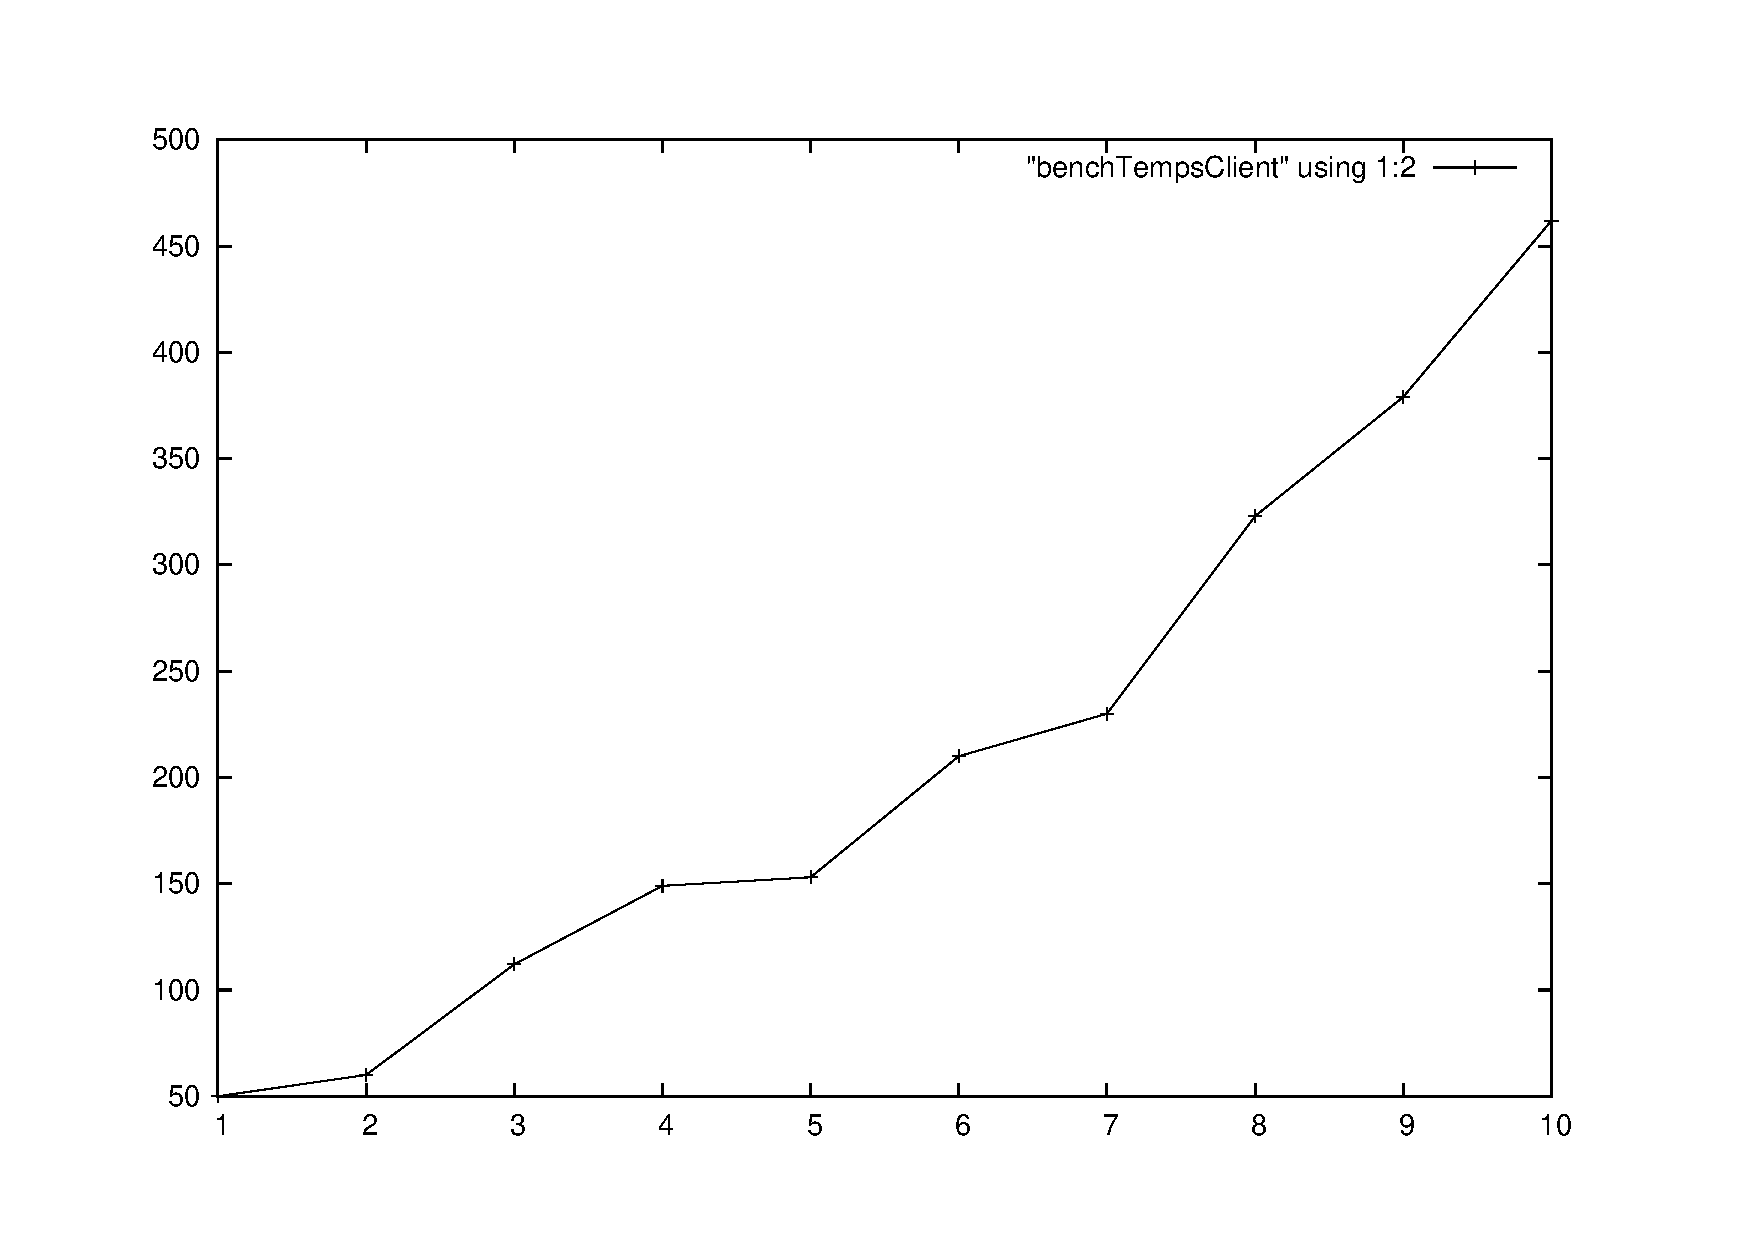
\includegraphics[scale=0.5]{src/benchTempsClient}
  \caption{Temps moyen d'execution du transaction en fonction du nombre de client}
\end{figure}

\subsubsection{Charge ciblant deux stores}
\paragraph{}
Nous avons la même architecture que dans le cas du dessus, à l'exception que nous nous retrouvons avec deux stores avec la moitié des threads effectuant des opérations sur l'un des stores et l'autre moitié sur l'autre store.
On observe que lorsque les dix threads sont lancés, nous obtenons les mêmes vitesses d'executions que dans le cas où cinq threads sont executés sur un seul store, ce qui parait logique car c'est l'equivalent du cas précédent avec deux machines.
\\
\\
\begin{tabular}{|c|c|}
    \hline
    Nombre de threads & Temsp d'execution moyen \tabularnewline
    \hline
    1 & 45 \tabularnewline
    2 & 46 \tabularnewline
    3 & 73 \tabularnewline
    4 & 132 \tabularnewline
    5 & 198 \tabularnewline
    \hline
 \end{tabular}

\subsection{Catalogue}

\paragraph{}
A partir de cette partie, nous développons notre application de façon distribué. Chaque KVDB que nous aurons seront géré chacun par un serveur. Nous avons decidé d'implementé une couche d'abstraction appelé "Gateway", qui s'occupera de recevoir les requètes et de retourner les resultats au client. Le Gateway possede connaissance de la localisation de chacun des profils, ainsi que leur tailles, et la taille des KVDB. Ainsi il aura la capacité de determiner sur quel Serveur un profile doit etre migré, lorsque celui ci est surchargé.
Finalement, le client ne connaitra que l'adresse du "gateway" et executera les opérations sur les profils à travers celui là.
L'ensemble de l'application communique grâce à l'API RMI.

Pour l'implementation de cette solution, nous avons donc eu besoin que le Gateway possede une base de donnée mise à jour regulièrement possedant :
\begin{itemize}
\item Une map "mapServeur" des serveurs en fonction des profils. Cette map permet de savoir avec quel serveur rmi nous devons discuter pour trouver le profil.
\item Une map "mapProfile" du nombre d'objets en fonction d'un profil. Cette map permet de savoir le nombre d'objets actuellement present dans le profil.
\item Une map "confServeur" avec les informations du KVStore en fonction du serveurRmi. Cette map permet de migrer les donnée d'un KVStore à un autre sans avoir à repasser par le Gateway.
\item Une map "serveurSize" du nombre d'objets en fonction du serveur. Cette map permet de verifier la charge d'un serveur.
\end{itemize}

Nous avont par ailleur créé la methode "IServeur needsMigration(IServeur serv,String profil)" qui observe la charge de tous les serveurs et la compare à la charge du serveur qui possede actuellement le profil.
Si jamais il trouve un serveur qui à 2fois moins d'objets que lui, et que l'ajout de ce nouveau profil ne risque pas de simplement inverser la charge. Alors il retourne ce Serveur qui servira de destination pour la migration.

Grace à ces differents procedés, la totalité des problematiques algorithmiques sont alors à traiter dans le Gateway. Les serveurs possedent les fonctions permetant les actions atomiques simple et les clients possedent les fonctionnalités avancés. Nous avons consideré que ce Design-Pattern était interessant car il permettait de regrouper toutes les complexité algorithmiques dans la même classe Java. Ainsi, en cas de mise à jour du produit final, les fonctionnalités Client restent opperationnelles car elle ne sont que des liens vers un interface. Ceci permet d'éviter d'enclancher des mise à jour lourdes sur tous les clients lors de la modification d'une fonction d'affichage.
De même, les serveurs ne possedant que les fonctions atomiques de bases, sont donc beaucoup moins appellé à subir des modifications.
Ainsi, grace à ce Design-Pattern en cas d'évolution du code dans un monde fonctionnel, les clients et les serveurs n'auraient pas besoin de subir un nouveau déploiment et seul le Gateway qui est un objet unique devrais alors subir des modification.

Un autre avantage du catalogue sous forme de Gateway est l'abstraction qu'il offre au client. Le client n'ayant aucune vision du fonctionnement coté serveur, il peut utiliser la Base De Donnée Repartie au même titre que s'il utilisais une Base locale. Avec la simple connaissance des ID de ses profils, il peut alors effectuer les opperations qu'il souhaite, en deleguant la totalité du travail au Gateway. Ceci offre la possibilité d'ajouter des optimisations tel que l'ajout de serveurs à la volée, ou à une gestion de la replication, sans jamais avoir besoin de modifier le Client.
Cet interface boite noire permet une isolation totale des données serveur et permet donc d'obtenir une plus grande sécurité vis à vis de la localisation des données par un tier, tout en permetant au Gateway d'avoir une plus grande liberté sur les actions possible. 

\subsection{Déplacement}

\paragraph{}
Notre politique de déplacement est de regarder, après chaque requète, si la base de données sur laquelle la requète n'est pas au moins deux fois plus grosse qu'une autre. Si c'est le cas, alors on migre le profil sur lequel on a fait les opérations sur le nouveau serveur.

Plus précisement :

La methode "IServeur needsMigration(IServeur serv,String profil)" du Gateway est appelé à chaque fois que nous appelons la fonction "int comit(int profile,boolean migrate)" avec la migration activée. Si le retour n'est pas nul, alors il existe un serveur sur lequel il peut etre interessant de migrer les données. La fonction appele alors "int migrate(String profile, IServeur serveurDest)" qui lance la migration a partir du serveur.
Une fois la migration effectué alors le Gateway envoi au serveur une demande de suppression de la donnée pour eviter les doublons. Il met ensuite à jour les differentes valeurs stoqué dans les map.
Du coté serveur, lorsque la fonction "migration(String profile,String[] kvstore, int lastObjetId)" est appelé alors le serveur creer une transaction qui aura pour but de recuperer toutes les données du profil sur le KVStore et de les copier sur un autre KVStore. La decision de suppression des ancienes données est faite par le Gateway après avoir vérifié que l'opération s'est bien déroulée.

Dans le but de garantir la coherence des données, nous avons decidé d'utiliser un verou uniquement pour l'utilisation des methodes de migration, du coté gateway et du coté serveur, nous avons egalement choisi de verouiller la hashmap "mapServeur", ainsi nous avons la garantie que lorsqu'un thread client executé sur le Gateway tente d'acceder à un serveur grace à son profil, alors ce thread aura toujours le lien vers le serveur qui possede la donnée. Les problemes d'acces concurent à une donnée sont donc uniquement à traiter lors des ajouts dans le KVStore et se retrouvent simplifié à un problème de concurence basique. 

L'avantage de cette solution est que du coté client, la totalité de ces interations sont invisibles. Le client ne possède que la connaissance des numéros de profils. La localisation de la donnée et la prise de decision d'une migration est faite par le Gateway. C'est egalement lui qui s'occupera de gerer toutes les requetes adressées aux serveurs.

L'interface client épuré ne possede donc que les actions relatives à ajouter un profil, supprimer un profil ou afficher un profil, ainsi que les methodes reprenant les fonctionnalités demandés tel que etape1, peupler ou meme producteur et consomateur.

\subsection {Multiclés}

Pour les transaction sur plusieurs profils venants de differents KVStore, nous avons décidé d'observer la charge de tous les Stores impliqué et de migrer toutes les données vers ce dernier, pour ensuite executer toutes les transactions sur le meme KVStore.

Plus précisement :

A partir du Gateway, la methode "int comitMultiCle(int[] profiles)" va observer la charge des differents serveurs grace à la map "mapServeur" en prenant le premier serveur en reference. Une fois ce serveur trouvé elle va alors declancher la migration de tous les profils vers son KVStore. Puis finalement elle va exectuer les transactions sur chacun de ces profils. Ne monopolisant alors qu'un seul KVStore pour cette liste d'opperations.

L'avantage de cette solution est que du coté serveur, la transaction multiclé n'est percu que comme une suite d'actions atomiques; "migrate" puis "commit".
Deplus du coté client, la transaction multiclé n'est vu que comme une liste d'opperations. L'abstraction créée par le Gateway permet de n'avoir que cette classe à modifier pour pouvoir creer des fonctionnalités complexes.


